\documentclass[presentation]{beamer}
\usepackage{common}
\usepackage{arydshln}

\newcommand{\cscat}[1]{$\langle\text{{\itshape#1}}\rangle$}
\newcommand{\csopt}[1]{{\itshape[#1]}}
\newcommand{\csalt}[1]{{\itshape(#1)}}
\newcommand{\op}[1]{\alert{`\texttt{#1}'}}
\newcommand{\operand}[1][\ldots]{{\normalcolor#1}}
\newcommand{\literal}[1]{\texttt{\alert{#1}}}
\newcommand{\bs}{$\backslash$}

\title[\lecturecode{C\#}]{Object-oriented programming in C\#}



\begin{document}

\AtBeginSubsection[]{
\frame{
\frametitle{Outline}
{\scriptsize{\tableofcontents[currentsection,currentsubsection,hideothersubsections,subsectionstyle=show/shaded/hide]}}
}
}

\frame[label=coverpage]{\titlepage}

%\fr{Outline}{
%  \bl{Parts}{\en{
%    \item Basic OO concepts in C\#
%    \item Some specific C\#/.NET mechanisms
%    \item Encapsulation, interfaces
%    \item Inheritance
%    \item Generics
%    \item Exceptions and some key C\# libraries
%    \item Functional programming in C\#
%    \item Other programming mechanisms
%  }}
%}

\section{Basic OO in C\#}
\newcommand{\codepath}[1]{../../code/lecture-01/#1}

\subsection{C\# and .NET}

\frs{5}{Brief introduction to C\#}{
  \bl{C\# and .NET}{\iz{
    \item Designed by Anders Hejlsberg around 2000 at Microsoft
    \item Is part of the .NET initiative, designed to compile over the Common Language Infrastructure (CLI)
    \item Current version is 10.0, released in 2021 for .NET 6.0
    \item Mono is a free, open-source compiler and runtime environment
    \item Initially developed as very similar to Java, then somewhat diverged
    \item Essentially, C\# took a different path than Java in following Scala
    \item Shall in these slides refer to ``mainstream/standard OOP'' to mean the intersection of Java/C\#
    }}
}

\frs{5}{.NET}{
  \bl{Main elements}{\iz{
    \item .NET started as a polyglot framework since its beginning
    \item C\# is by far the mostly used language
    \item Concepts replicate Java and JVM: CIL/bytecode, CLR/JVM, and so on
    \item As a key difference, .NET initially targeted Microsoft Windows
    }}
  \fg{height = 0.4\textheight}{img/dotnet-overview.pdf}
}


\begin{frame}{\dotnet Platform -- Present vs. Past}
 \bl{Past to Present}{\iz{
        \item Before \dotnet 5 there used to be three major implementations of the \emph{class library}:
        %
        \begin{description}
            \item[\dotnet Framework] | Windows-specific, full-featured, targetting desktop and web applications
            \item[\dotnet Core] | multi-platform (Win, Mac, Linux), less-featured, targetting desktop and web applications
            \item[Xamarin] | mobile-oriented (Android, iOS, Mac OS) 
        \end{description}

        \vfill

        \item Since \dotnet 5, implementations are aligned
    }}
    \bl{In these slides}{
        Stick to \alert{\dotnet Core 3.1}, to maximise interoperability and to avoid compatibility issues
    }
\end{frame}


\frs{20}{Features of C\#}{
  \bl{Ingredients}{\iz{
    \item C-like language: the imperative and structured parts are very similar
    \item Java-like language: essentially very similar to Java, specially at the beginning
    \item Static and strong typing: types are checked at run-time, preventing ill-typed operations
    \item Object-orientation: object by references, automatic garbage collection
    \item Functional-orientation: generics, delegates, lambdas
    }}
  \bl{Philosophy}{\iz{
    \item aiming at high expressiveness and richness, though become a rather ``large'' language
  }}
  \fg{height = 0.4\textheight}{img/sizes.png}
}


\fr{C\# types: we start with Simple Types and Class Types}{
  \fg{height = 0.6\textheight}{img/type-system.pdf}
}
  
\frs{20}{Variables: initialisation and inference}{
  \bl{On variables -- essentially as in Java}{\iz{
  \item Same rules on scoping, and assignment
  \item Similar distinction between primitive and class types
  \item Similar naming conventions for variables
  \item \texttt{null} is assignable to variables of reference types
  \item Can use \texttt{var} to declare a variable with type to be inferred
  \item Keywords (\cil{int}, \cil{bool}, \cil{string}, \cil{object}) map to Library Value Types or Classes
  }}
  \codeview{3}{9}{24}{\scriptsize}{\codepath{InitialExamples/Initialisation.cs}}
}

\begin{frame}{\dotnet Built-in Types}\centering
    \begin{table}[]
        \resizebox{\textwidth}{!}{
        \begin{tabular}{c|c|c|c|c}
            \textbf{Name}    & \textbf{Keyword} & \textbf{Category} & \textbf{Size} & \textbf{Description}  \\
            \hline\hline
            \texttt{Boolean} & \texttt{bool}    & \emph{val} & 1             & either \texttt{true} or \texttt{false} \\
            \texttt{Char}    & \texttt{char}    & \emph{val} & 2             & UTF-16 characters \texttt{`U+0000'} \ldots \texttt{`U+FFFF'} \\
            \texttt{Byte}    & \texttt{byte}    & \emph{val} & 1             & integers in $0 \ldots (2^{8}-1)$ \\
            \texttt{SByte}   & \texttt{sbyte}   & \emph{val} & 1             & integers in $-2^{7} \ldots (2^{7}-1)$ \\
            \texttt{Int16}   & \texttt{short}   & \emph{val} & 2             & integers in $-2^{15} \ldots (2^{15}-1)$ \\
            \texttt{UInt16}  & \texttt{ushort}  & \emph{val} & 2             & integers in $0 \ldots (2^{16}-1)$ \\
            \texttt{Int32}   & \texttt{int}     & \emph{val} & 4             & integers in $-2^{31} \ldots (2^{31}-1)$ \\
            \texttt{UInt32}  & \texttt{uint}    & \emph{val} & 4             & integers in $0 \ldots (2^{32}-1)$ \\
            \texttt{Int64}   & \texttt{long}    & \emph{val} & 8             & integers in $-2^{63} \ldots (2^{63}-1)$ \\
            \texttt{UInt64}  & \texttt{ulong}   & \emph{val} & 8             & integers in $0 \ldots (2^{64}-1)$ \\
            \texttt{Float}   & \texttt{float}   & \emph{val} & 4             & abs in $1.5\times 10^{-45} \ldots 3.4\times 10^{38}$ \\
            \texttt{Double}  & \texttt{double}  & \emph{val} & 8             & abs in $5.0\times 10^{-324} \ldots 1.7\times 10^{308}$ \\
            \texttt{Decimal} & \texttt{decimal} & \emph{val} & 16            & abs in $1.0\times 10^{-28} \ldots 7.9228 \times 10^{28}$ \\
            \texttt{Object}  & \texttt{object}  & \emph{ref} & O(1)          & anything \\
            \texttt{String}  & \texttt{string}  & \emph{ref} & O($n$)   & sequences of $n$ UTF-16 characters \\
        \end{tabular}
        }
    \end{table}

    \tiny
    (cf. \url{https://docs.microsoft.com/dotnet/csharp/language-reference/builtin-types/built-in-types})
\end{frame}

\subsection{Basic OOP}


\frs{5}{C\# classes}{
  \bl{The core of OOP is essentially as in Java} {\iz{
    \item Classes, methods, fields, and constructors have same syntax and semantics
    \item Class instantiation, method invocation, field access have same syntax and semantics
    \item Static, non-static fields/methods have same syntax/semantics
    \item Structured programming constructs (if/while) have same syntax/semantics
    \item A source file must define the namespace, similar to Java package but in a wrapping construct
    \item Syntax for calling a constructor from another constructor is different
  }}
  \bl{Formatting}{\iz{
    \item Slightly different conventions on formatting braces 
    \item Methods start with an uppercase, fields with an underscore
    \item \myurl {https://docs.microsoft.com/en-us/dotnet/csharp/programming-guide/inside-a-program/coding-conventions}
  }}
}

\frs{5}{\Cil{Point3D}}{
\codeview{0}{2}{34}{\tiny}{\codepath{Point3D/Program.cs}}
}

\fr {C\# executable programs} {
   \bl {Building blocks of C\# software} {\iz {
     \item class libraries shipped with .NET
     \item possibly other external libraries 
     \item a set of classes that make up the application we build (like \cil{Point3D)}
     \item at least one of these classes has a special method \cil{Main}
     \item a \cil {Main} is the entry point of a program
   }}
   \bl{The \cil {Main} must have the following declaration: }{\iz {
   \item \cil {public static void Main() \{.. \}}
    \item there could be variant with different inputs, outputs, and visibility, but we won't see them now
    \item it is key it is call \cil{Main} and is \cil{static}
    \item \cil{static} means this method is ``shared'' among all objects, and is conceptually called to the class, not to the object
   }}
}

\frs{15}{Typical structure of an executable project} {
   \bl{Entry point class} {\iz {
     \item it contains the \cil{Main} method
     \item typically, it contains only that method
   }}
   \bl{Other classes}{\iz{
     \item contain the various application classes
   }}
   \bl{Source files}{\iz{
    \item have \cil{.cs} extension
    \item start with ``\cil{using}'' clauses to declare other classes they use
    \item declared one or more classes, enclosing them in \cil{namespace}s
    \item a \cil{namespace} is a ``module'' giving a context to the class
   }}
   \bl{Project}{\iz{
    \item has a name
    \item has one or many sources
    \item specify additional properties, and dependencies (references to other projects)
   }}
}

\fr{A class \Cil{Person}}{
\codeview{1}{5}{34}{\tiny}{\codepath{Person/Program.cs}}
}

\frs{10}{Constructors chaining}{
\codeview{1}{5}{37}{\tiny}{\codepath{PersonChaining/Program.cs}}
}

\frs{10}{Playing with libraries (namespace \Cil{System})}{
\codeviewall{\tiny}{\codepath{PlayWithLibraries/Program.cs}}
}

\frs{10}{State, Getters and Setters}{
    \bl{An object state}{\iz{
        \item an object carries a state, in the form of a structure set of data
        \item internally this is represented by a set of named and typed fields, which are private
        \item externally this is represented by a set of named and typed ``properties''
        \item such properties may or may not overlap with fields
        \item to make such properties accessible to clients, specific methods are needed
    }}
    \bl{Getters and Setters}{\iz{
        \item a common solution in OOP (will see C\# will improve it)
        \item a getter is method \cil{GetXYZ} with 0-args, returning the property \cil{XYZ}'s value, and typically causing no side-effect
        \item a getter is a method \cil{SetXYZ} taking the property \cil{XYZ}'s value and returning nothing
        \item properties that one only wants to read have no setter, and vice-versa for getters
    }}
}

\frs{5}{\Cil{Person} with Getters and Setters}{
\codeview{1}{18}{48}{\tiny}{\codepath{PersonGetters/Program.cs}}
}

\fr{Client code for \Cil{Person}}{
\codeview{2}{7}{16}{\scriptsize}{\codepath{PersonGetters/Program.cs}}
}

\fr{Expression-bodied members}{
    \bl{Syntax: \texttt{<member> => expression; }}{\iz{
        \item can be used for methods and constructors
        \item when their body is a single return of an expression, or just a single statement...
        \item you can directly indicate the signature, \texttt{=>}, and that expression/statement
        \item it makes your programs more short and readable: use them!
    }}
}

\fr{\Cil{Person} with Expression-bodied methods}{
\codeview{1}{18}{39}{\ssmall}{\codepath{PersonExpBody/Program.cs}}
}

\fr{Immutability}{
    \bl{Design for immutability}{\iz{
        \item by choosing which property has a Setter we can decide that there is information that cannot be changed, and this is important to avoid clients to badly affect the behaviour of our objects
    }}
    \bl{Readonly fields}{\iz{
        \item the same has to be done for fields: if a field is initialised at construction time and then never changed, we shall use modifier \cil{readonly}
        \item this enhance clarity of programs, and the compiler check we do not alter such fields
    }}
}


\frs{15}{Properties}{
    \bl{Improving over Get/Set accessors}{\iz{
        \item C\# introduces a programming construct for properties
        \item a property is directly perceived by the client as a sort of field (starting with uppercase)
        \item internally to a class, a property is actually a getter and/or setter with special syntax
    }}
    \bl{Notation}{\iz{
        \item \cil{public <type> <name>\{ get \{...\} set \{...\} \}}
        \item the body of \cil{get} should return a value
        \item the body of \cil{set} can use a special variable \cil{value}
        \item for both we can use expression-bodied get/set
        \item \cil{get} or \cil{set} could be private
        \item can use expression-bodied readonly property in one line
    }}
    \bl{The special case of auto-implemented properties}{\iz{
        \item if the body of \cil{get} and \cil{set} are entirely skipped, a field with same name of the property is implicitly defined
    }}
}

\fr{\Cil{Person} with Properties}{
\codeview{1}{5}{33}{\tiny}{\codepath{PersonProperties/Program.cs}}
}

\frs{5}{\Cil{Person} with Properties: playing with properties}{
\codeview{1}{20}{50}{\tiny}{\codepath{PersonPropertiesPlay/Program.cs}}
}

\fr{Playing with properties: client code}{
\codeview{2}{7}{18}{\scriptsize}{\codepath{PersonPropertiesPlay/Program.cs}}
}

\section{Some specific C\# mechanisms}
\renewcommand{\codepath}[1]{../../code/lecture-02/#1}

\subsection{Arrays}

\begin{frame}{\dotnet Arrays}
    \begin{block}{Array types}
        \begin{description}
            \item[\texttt{\textit{T}\alert{[]}}] denotes the \alert{array of \texttt{\textit{T}}} type
            \item[\texttt{\textit{T}\alert{[][]}}] denotes the \alert{array of \emph{arrays of} \texttt{\textit{T}}} type
            \item[\texttt{\textit{T}\alert{[][][]}}] denotes the \alert{array of \emph{arrays of arrays of} \texttt{\textit{T}}} type
            \item[\texttt{\textit{T}\alert{[][,]}}] denotes the \alert{array of \emph{2-dimensional arrays of} \texttt{\textit{T}}} type
            \item[\texttt{\textit{T}\alert{[,,][]}}] denotes the \alert{3-dimensional array of \emph{arrays of} \texttt{\textit{T}}} type
        \end{description}
    \end{block}
\end{frame}
\begin{frame}[shrink=5]{\dotnet Arrays}
    \begin{block}{Arrays features}
        \begin{itemize}
            \item All array types are \alert{reference} types
            %
            \begin{itemize}
                \item arrays of value types are reference types as well
            \end{itemize}

            \item All array types are subtypes of the \texttt{Array} class

            \item Arrays are constructed by sizes, i.e. $D_1, \ldots, D_N$ are user-provided
            %
            \begin{itemize}
                \item so memory can be contiguously allocated
                \item items are initialised to their default values
            \end{itemize}

            \item All array types come with 3 useful properties/methods:
            %
            \begin{description}
                \item[\texttt{Rank}] returning the total amount of dimensions of the array (i.e. $N$)
                \item[\texttt{Length}] returning the total amount of items in the array (i.e. $D_1 \times \ldots \times D_N$)
                \item[\texttt{GetLength($i$)}] returning the total amount of items along the $i$-th dimension (i.e. $D_i$)
            \end{description}

            \item Access to items is performed via the indexed-access operator:
            %
            \begin{center}
                \op{\operand[array][\operand[index$_1$, \ldots, index$_N$]]}  
            \end{center}
        \end{itemize}
    \end{block}
\end{frame} 

\begin{frame}[allowframebreaks]{Array Types Instantiation}
    \begin{block}{Constructors for $N$-dimensional Arrays of \texttt{\textit{T}}}
        \begin{center}\ttfamily
            \textit{T}[\alert{,,}\ldots{}] \cscat{Var Name} = \alert{new} \textit{T}[\alert{$D_1$}, \alert{$D_2$}, \ldots];
        \end{center}
        %
        \begin{itemize}
            \item Number of commas in the left-hand side: $N-1$
            \item Number of sizes in the right-hand side: $N$
        \end{itemize}
    \end{block}
    \begin{block}{Literal Array Expressions for $N$-dimensional Arrays of \texttt{\textit{T}}}
        \begin{center}\ttfamily
            \textit{T}[\alert{,,}\ldots{}] \cscat{Var Name} = \alert{new} \textit{T}[\alert{,,}\ldots{}] 
                \alert{\{\ldots\{} \cscat{Item$_1$}, \cscat{Item$_2$}, \ldots  \alert{\}\ldots\}};
        \end{center}
        %
        \begin{itemize}
            \item Number of commas in the left-hand side: $N-1$
            \item Number of nesting levels of braces in the right-hand side: $N$
            \item Repeating \texttt{\textit{T}[\alert{,,}\ldots{}]} may be avoided in the right-hand side
        \end{itemize}
    \end{block}

    \framebreak
    
    \codeview{3}{9}{24}{\tiny}{\codepath{Snippets/Snippet6Arrays.cs}}

\end{frame}

\begin{frame}[allowframebreaks]{Accessing Arrays Items}
    \codeview{2}{27}{41}{\tiny}{\codepath{Snippets/Snippet6Arrays.cs}}

    \codeview{2}{43}{52}{\tiny}{\codepath{Snippets/Snippet6Arrays.cs}}

\end{frame}

\subsection{Nullables}

\begin{frame}[shrink=5]{\dotnet Nullables}
    \bl{Nullable types definition}{\iz{
        \item let \texttt{\textit{T}} by a \alert{value} type of any sort, then \texttt{\textit{T}\alert{?}} denotes the \alert{nullable \texttt{\textit{T}}} type

        \item A nullable type \texttt{\textit{T}?} can be defined as \texttt{\textit{T}} $\cup$ \{ \texttt{null} \}.
        %
        \item A variable of type \texttt{\textit{T}?} can be assigned with any admissible value of \texttt{\textit{T}}, \alert{or} with \texttt{null}
        }
        
        {\tiny (cf. \url{https://docs.microsoft.com/dotnet/csharp/language-reference/builtin-types/nullable-value-types})}
    }
    \begin{block}{Nullables features}
        \begin{itemize}
            \item All nullable types are \alert{value} types

            \item The notation \texttt{\textit{T}?} is another way of writing \texttt{Nullable<\textit{T}>}
            %
            \item All nullable types come with some useful properties:
            %
            \begin{description}
                \item[\texttt{HasValue}] returning null if the object is null
                \item[\texttt{Value}] returning the non-null value, if present
            \end{description}

            \item When non-null, nullable-type variables behave like they non-nullable counterparts
        \end{itemize}
    \end{block}
    
\end{frame}

\begin{frame}{Nullable Types Operators}
    \begin{block}{}
        \begin{itemize}
            \item Operator \cil{??} gets the value or a default if null

            \item Operator \cil{?.} calls a method on a nullable only if not null, otherwise it does nothing and yields null
        \end{itemize}
    \end{block}

    \codeview{3}{9}{19}{\scriptsize}{\codepath{Snippets/Snippet7Nullables.cs}}
\end{frame}

\section{Encapsulation, interfaces}
\renewcommand{\codepath}[1]{../../code/lecture-03/#1}

\subsection{Encapsulation, and properties}

\frs{5}{Encapsulation}{
  \bl{Two crucial ingredients of OO programming}{\en{
    \item Packing data + functions to manipulate it
    \item Information hiding via careful access control
  }}
  \bl{Philosophy}{\iz{
    \item Each class declares \cil{public} only those (few) methods/properties/constructors necessary to interact with (or create) its instances
    \item The rest (which therefore includes mere implementation aspects) is \cil{private}{\iz{
      \item methods/constructors/properties for internal use only
      \item{\bf{all}} fields (i.e. internal status)
    }}
  }}
  \bl{Encapsulation and dependencies}{In this way the ``client'' is weakly influenced by possible future modifications concerning mere implementation aspects.
  }
}

\frs{5}{A basic case: class \Cil{Counter}}{
    \codeview{1}{18}{40}{\scriptsize}{\codepath{Counter/Program.cs}}
}

\fr{A basic case: usage of class \Cil{Counter}}{
    \codeview{1}{5}{16}{\scriptsize}{\codepath{Counter/Program.cs}}
}


\fr{Encapsulation is preserved by properties!}{
    \codeview{1}{5}{25}{\ssmall}{\codepath{CounterProperties/Program.cs}}
}

\fr{A transparent modification to the \Cil{Counter} implementation}{
    \codeview{1}{28}{47}{\ssmall}{\codepath{CounterProperties/Program.cs}}
}

\fr{A final bit on properties: object initializers}{
    \codeview{1}{5}{32}{\ssmall}{\codepath{ObjectInitializer/Program.cs}}
}

\fr{Properties vs methods vs fields: recap}{
    \bl{``Properties are just methods''}{\iz{
        \item a read-only property is essentially a Getter
        \item a read-write property is essentially a pair of Getter and Setter method
        \item most discussions in the following focus on methods, and applicability to properties naturally derive
    }}
    \bl{``Properties define a nice abstraction''}{\iz{
        \item from the design viewpoint, public properties are much nicer than Getters/Setters, which are still the OOP standard
    }}
    \bl{``Properties can replace fields''}{\iz{
        \item as an implementation mechanism, auto-implemented properties are a good replacement for fields
        \item but this is just matter of internal implementation
    }}
}

\subsection{Interfaces}


\frs{10}{C\# \Cil{interfaces}}{
  \bl{What is an \cil{interface}}{\iz{
    \item It is a new declarable \alert{reference type} (like classes)
    \item It has a name, and includes a set of method signatures (and properties)
    \item It cannot be used to create objects the \cil{new} operator
  }}
  \bl{An \cil{interface} \cil{I} can be ``implemented'' by a class}{\iz{
    \item Through a class \cil{C} that explicitly declares it (\cil{class C : I \{.. \}})
    \item \cil{C} will define (the body of) all methods declared in \cil{I}
    \item An instance object of \cil{C}, will have the usual \cil{C} type, but also \cil{I}
    \item namely, type \cil{C} is a subtype of \cil{I}
    \item C\# convention for interface names: \cil{IDevice}, \cil{IPerson}, \dots
    \item later versions of C\# provide default methods for interfaces
  }}
  \bl{Substitutability}{\iz{
    \item As usual in OOP: an object created by a class implementing an interface can be passed to where an element of the interface is expected
  }}
}

\fr{Interface \Cil{IDevice}}{
\bx{\cil{IDevice} introduce a contract for devices: they provide services to be switched on, switched off, and to check if they are on.}
\codeview{1}{5}{12}{\small}{\codepath{SmartHome/Program.cs}}
}

\frs{5}{Two lamp implementations of \Cil{Device}}{
  \codeview{1}{14}{38}{\ssmall}{\codepath{SmartHome/Program.cs}}
}

\frs{5}{Multiple implementation}{
  \bl{Multiple implementation}{Possible declaration: \cil{class C : I1, I2, I3 \{.. \}}
  \iz{
    \item A class \cil{C}  implements \cil{I1} and \cil{I2} and \cil{I3}
    \item The class \cil{C}  ust provide a body for all methods of \cil{I1}, all those of \cil{I2}, all those of \cil{I3}{\iz{
      \item if \cil{I1}, \cil{I2}, \cil{I3} had common methods there would be no problem, each one should be implemented only once
    }}
    \item Instances of \cil{C} have type \cil{C}, but also types \cil{I1}, \cil{I2} and \cil{I3}
  }}
  \bl{Extension}{Possible declaration: \cil{interface I : I1, I2, I3 \{.. \}}
  \iz{
    \item An interface \cil{I} defines certain methods, in addition to those of \cil{I1}, \cil{I2}, \cil{I3}
    \item A class \cil{C} that implements \cil{I} must provide a body for all methods indicated in \cil{I}, plus all those of \cil{I1}, all those of \cil{I2}, and all those of \cil{I3}
    \item Instances of \cil{C} have type \cil{C}, but also types \cil{I}, \cil{I1}, \cil{I2} and \cil{I3}
  }}
}

\section{Inheritance}
\renewcommand{\codepath}[1]{../../code/lecture-04/#1}

\subsection{Class extension}

\fr{Inheritance}{
  \bx{
    It is a mechanism that allows you to define a new class \alert{specialising} an existing one, that is, ``inheriting'' its members (the private ones are not directly visible), possibly modifying / adding new members, and therefore reusing code already written and tested.
  }
  \bl{Inheritance is a key concept of OOP}{\iz{
    \item It is related to the interface mechanism
    \item It is one of the key elements along with encapsulation and interfaces
    \item It not only affects code reuse, but also the resulting polymorphism
  }}
  \bl{Abstract classes}{\iz{
    \item dealt with in a completely standard way, we won't consider them further here
  }}
}


\fr{Basic example: \Cil{Counter}}{
\codeview{1}{5}{25}{\scriptsize}{\codepath{Counter/Program.cs}}
}

\frs{15}{The need to extend and modify}{
  \bl{The inheritance mechanism can be used for a multicounter}{\iz{
    \item Definition: \cil{class C : D \{.. \}}
    \item The new \cil{C} class inherits all members of \cil{D}{\iz{
      \item The private members are not directly accessible from within \cil{C}
      \item The constructors of \cil{D} must always be rewritten, and should properly call \cil{C}'s
      \item The constructor of a subclass should have the \cil{base} statement, which calls a (non-private) constructor of the parent class
    }}
  }}
  \codeview{1}{18}{29}{\scriptsize}{\codepath{MultiCounterInheritance/Program.cs}}
}


\frs{8}{\Cil{protected} access level }{
  \bl{Usable for the members of a class}{\iz{
    \item It is an intermediate level between \cil{public} and \cil{private}
    \item Indicates that the member (field, method, constructor, property) is accessible from the current class, from a subclass, and from subclasses of subclasses (recursively)
  }}
  \bl{What is it for?}{\iz{
    \item It allows subclasses to access supra-class information that you don't want clients to see
    \item Most often used in retrospect replacing a \cil{private}
    \item Using \cil{protected} fields is to be avoided -- it somewhat breaks encapsulation; should better use \cil{protected} properties/methods
  }}
  \bl{Example class \cil{BiCounter} - bidirectional counter}{\iz{
    \item A counter with also the \cil{Decrement} method
    \item Impossible without making the \cil{Value} accessible also for modification
  }}
}

\fr{\Cil{ExtendibleCounter} and \Cil{BiCounter}}{
  \codeview{1}{5}{34}{\tiny}{\codepath{BiCounter/Program.cs}}
}

\fr{Analogous solution with fields}{
  \codeview{1}{18}{38}{\ssmall}{\codepath{BiCounterFields/Program.cs}}
}

\frs{20}{Overriding}{
  \bl{Extension and modification}{\iz{
    \item When creating a new class by extension, it is very often not enough to add new functionality
    \item Sometimes it is also necessary to modify some of those available, possibly even distorting a bit their original functioning
    \item This can be done by rewriting in the subclass one (or more) of the methods/properties of the superclass -- called an \alert{override}
    \item To do so, methods/properties in the base class must be declared \cil{virtual}, and those in the subclass \cil{override}
    \item If necessary, the rewritten method can invoke the version of the parent using the special receiver \cil{base}
    \item It is possible to ``hide'' a method in the superclass that is not \cil{virtual}, by the modifier \cil{new} -- but this mechanis is optional, and arguably with limited use
    \item A class can be declared \cil{sealed} to prevent extension
    
  }}
  \bl{Example \cil{LimitCounter}}{\iz{
    \item Create a (sealed) counter which, having reached a certain limit, no longer continues
    \item It is necessary to override the \cil{Increment()} method
    \item An additional getter method inspects when the limit is reached
  }}
}

\fr{Using the \Cil{LimitCounter} class}{
  \codeview{1}{5}{18}{\scriptsize}{\codepath{LimitCounter/Program.cs}}
}


\fr{Class \Cil{LimitCounter}}{
  \codeview{1}{20}{41}{\scriptsize}{\codepath{LimitCounter/Program.cs}}
}

\fr{A summary of access modifiers (for types and members)}{
    \bx{Recall that \cil{internal} means ``visible only in this assembly''}
    \bl{Who can access?}{\iz{
        \item \cil{public}: any other code in the same assembly or another assembly that references it
        \item \cil{private}: only by code in the same class
        \item \cil{protected}: only by code in the same class, or in a class that is derived from that class
        \item \cil{internal}: by any code in the same assembly, but not from another assembly
        \item \cil{protected internal}: by any code in the assembly in which it's declared, or from within a derived class in another assembly
        \item \cil{private protected}: only within its declaring assembly, by code in the same class or in a type that is derived from that class
    }}
}

\fr{Class \Cil{Object}}{
    \bl{Implicit extension of \cil{Object}}{\iz{
        \item when a class extends nothing, it is like extending \cil{System.Object}
        \item transitively, this means all classes inherit from \cil{Object}
        \item it provides low-level services for all objects 
        \item we will in the following explain some of them
    }}
    \bl{Method \cil{String ToString()}}{\iz{
        \item it can be overriden to provide a canonical string representation of an object
        \item \cil{Console.Write} uses it if you try to write an object
    }}
}

\subsection{Runtime types}

\fr{Polymorphism with \Cil{object}}{
  \codeview{1}{5}{29}{\ssmall}{\codepath{PolyObject/Program.cs}}
}


\fr{\Cil{UsePerson} and \Cil{Person}}{
  \codeview{1}{5}{34}{\tiny}{\codepath{Person/Program.cs}}
}

\fr{Specialisations of \Cil{Person}}{
  \codeview{1}{36}{58}{\tiny}{\codepath{Person/Program.cs}}
}

\frs{5}{Static type and run-time type}{
  \bl{A duality introduced by subtyping (inclusive polymorphism)}{\iz{
    \item Static type: the data type of an expression that can be inferred by the compiler
    \item Run-time type: the data type of the value (/ object) actually present (could be a subtype of the static one, and can be inspected with \cil{GetType()}){\iz{\item in this case virtual method calls rely on late-binding}}
  }}
  \bl{Example in \cil{PrintAll()} code, inside the \cil{foreach}}{\iz{
    \item Static type of \cil{obj} is \cil{Object}
    \item Run-time type of \cil{obj} varies from time to time: \cil{String}, \cil{Int32}, \dots
  }}
  \bl{Type inspection at run-time}{\iz{
    \item In some cases it is necessary to inspect the type at run-time
    \item The case of the \cil{is} and \cil{as} operators
    \item However, using them is bad practice: it means you have poorly used polymorphism
  }}
}

\fr{Type check and conversion}{
  \codeview{1}{6}{32}{\tiny}{\codepath{PersonRuntime/Program.cs}}
}

\section{Generics}
\renewcommand{\codepath}[1]{../../code/lecture-05/#1}

\subsection{Generic classes}

\fr{Uniform abstractions with classes}{
  \bl{Uniform abstractions for recurring problems}{\iz{
    \item During the development of various systems, recurrent problems are encountered that can find a common solution
    \item In some cases these solutions are factorisable (by abstraction) into a single highly reusable class
  }}
  \bl{A fundamental case: the \alert{collection}}{\iz{
    \item A collection is an object whose task is to store the reference to a (typically unspecified) number of other objects
    \item Among its tasks is to allow modifications and quick access to the set of elements of this collection
    \item Various strategies can be used, following the theory/practice of algorithms and data structures
  }}
}

\fr{Preliminary \Cil{UseIntVector}}{
  \codeview{1}{5}{21}{\scriptsize}{\codepath{IntVectorPre/Program.cs}}
}

\fr{Preliminary \Cil{IntVector}}{
  \codeview{1}{23}{53}{\tiny}{\codepath{IntVectorPre/Program.cs}}
}

\frs{5}{C\# Indexers}{
    \bl{Let's improve this design a bit}{\iz{
        \item we have getters/setters that are parametric, namely, they depend on an indexer
        \item we would like to handle them as we would with properties
    }}
   \bl{C\# Indexer}{\iz{
        \item a sort of parametric property
        \item it has no name 
        \item it supports the array access notation for reading and/or writing elements
        \item basic syntax: \cil{public <type> this[<type> <name>]\{ get\{...\} set\{...\}\}}
        \item could have many parameters of the indexer
        \item could have many indexers in a class, with different parameters
    }}
}

\frs{5}{\Cil{IntVector} (with indexer)}{
  \codeview{1}{19}{51}{\tiny}{\codepath{IntVector/Program.cs}}
}

\fr{\Cil{UseIntVector}}{
  \codeview{1}{5}{17}{\scriptsize}{\codepath{IntVector/Program.cs}}
  \bx{In this lesson we shall assume we never ``escape'' boundaries of arrays and collections, which would result in exceptions} 
}

\frs{5}{A first step towards uniformity}{
  \bl{Only vectors of \cil{int}?}{\iz{
    \item Experience would immediately lead to the need to design vectors of \cil{double}, \cil{bool}, \dots that is, of any value type
    \item And then, also vectors of \cil{String}, \cil{DateTime}, and so on
    \item The implementation would be similar, but without the possibility of reuse.
  }}
  \bl{The idea of ``monomorphic'' collections}{\iz{
    \item A first solution to the problem is obtained by exploiting inclusive polymorphism and the ``everything is an object'' philosophy (including the use of autoboxing)
    \item Only a \cil{ObjectVector} is created, simply by replacing \cil{int} with \cil{object}
    \item Any element is inserted (via implicit upcast conversions)
    \item When you get a value back you need an explicit downcast with \cil{as} operator
    \item Working with such interfaces gets bloated, and low-level
  }}
}

\fr{\Cil{UseObjectVector}}{
  \codeview{1}{5}{32}{\ssmall}{\codepath{ObjectVector/Program.cs}}
}

\frs{5}{\Cil{ObjectVector}}{
  \codeview{1}{34}{66}{\tiny}{\codepath{ObjectVector/Program.cs}}
}

\fr{Another example of collection: \Cil{ObjectList}}{
  \codeview{1}{25}{47}{\ssmall}{\codepath{ObjectList/Program.cs}}
}

\fr{\Cil{UseObjectList}}{
  \codeview{1}{6}{23}{\ssmall}{\codepath{ObjectList/Program.cs}}
}

\fr{The need for a parametric polymorphism approach}{
  \bl{In C\# 1.0}{\iz{
    \item This was the standard approach to building collections
  }}
  \bl{Problem}{\iz{
    \item With this approach, C\# code resulted in many uses of objects similar to \cil{ObjectVector} or \cil{ObjectList}
    \item It was very easy to lose track of what the content was \dots {\iz{
      \item which objects a collection contain? only \cil{int}? only \cil{strings}?
    }}
    \item The code often contained bad conversions
  }}
  \bl{More generally}{
    The problem arises every time I want to collect objects whose type is not known a priori, but could be subject to inclusive polymorphism
  }
}

\frs{5}{Parametric polymorphism}{
  \bl{Basic idea: generification}{\iz{
    \item Given a code snippet \cil{F} that works on a certain type, say \cil{string}, if it could also work uniformly with others\dots
    \item \dots you make it parametric by replacing \cil{string} with a sort of \cil{T} variable (called \alert{type-variable}, i.e. a variable that contains a type)
    \item At this point, when you need the code fragment instantiated on the strings, you use \cil{F<String>}, that is, it is required that \cil{T} becomes \cil{string}
    \item When you need the code snippet instantiated on integers, use \cil{F<int>}
  }}
  \bl{C\# Generics}{\iz{
    \item Generic classes / interfaces / methods
    \item Fully integrated in the type system and run-time (differently from other frameworks, like the JVM)
    \item Typical application with collections
  }}
}

\frs{5}{Generic vector}{
  \codeview{1}{33}{65}{\tiny}{\codepath{GenericVector/Program.cs}}
}

\fr{Using generic vector}{
  \codeview{1}{5}{31}{\ssmall}{\codepath{GenericVector/Program.cs}}
}

\subsection{Generic methods}

\fr{Generic Methods}{
  \bl{Basic idea}{\iz{
    \item generify a single method in the type(s) of some of its arguments/return
    \item syntactically: add type parameter after method name
    \item at the call side: specify type parameter after method name
    \item at the call side: use type inference, simply avoiding any specification
  }}
  \bl{Two typical applications}{\iz{
    \item generic static methods: as helpers working on generic structures
    \item in generic classes: as a helper to mix differen instantiations
  }}
  \bl{Syntax is ad-hoc}{\iz{
    \item type parameters come after method name in declarations/invocations
    \item type parameters in invocations can be inferred
  }}
}

\fr{Generic static methods}{
    \codeview{1}{7}{34}{\ssmall}{\codepath{GenericMethods/Program.cs}}
}

\fr{Generic instance methods: the case of class \Cil{Pair<TA,TB>}}{
  \codeview{1}{35}{51}{\ssmall}{\codepath{Pair/Program.cs}}
}

\fr{Using pairs}{
  \codeview{1}{6}{33}{\ssmall}{\codepath{Pair/Program.cs}}
}

\subsection{Generic interfaces}

\frs{10}{Generic interfaces}{
  \bl{What is a generic interface}{\iz{
    \item It is an interface that declares type-variables: \cil{interface I <T1, T2> \{.. \}}
    \item The type-variables appear in the methods signatures defined by the interface
    \item When a class implements it, it must instantiate the type variables (or assign them to other type-variables if it is generic)
  }}
  \bl{Uses}{
    To create uniform contracts that do not have to depend on the types used
  }
  \bl{Example 1}{\iz{
    \item An \cil{IGenericVector<T>} would be used to abstract over \cil{GenericVector<T>}
  }}
  \bl{Example 2: a new case, \alert{Iterators}}{\iz{
    \item An iterator is an object used to access a sequence of elements
    \item We will now look at a simplified version - different from that of the Java libraries
  }}
}

\fr{\Cil{IGenericVector<T>}}{
  \codeview{1}{20}{27}{\footnotesize}{\codepath{IGenericVector/Program.cs}}
}

\frs{5}{Implementing \Cil{IGenericVector}}{
  \codeview{1}{29}{61}{\tiny}{\codepath{IGenericVector/Program.cs}}
}

\subsection{Iterators and collections}

\frs{10}{The Iterator pattern}{
    \bl{Idea}{\iz{
        \item Assume an object represents a set of values {\iz{
            \item a collection, a source of information, a mathematical set,\dots
        }}
        \item \dots how could it give a service to let clients retrieve all such values?
        \item Iterator pattern: the object gives to requestors a so-called \alert{iterator}
        \item An iterator is an object with a method to extract the ``next'' element of the set, to be called iteratively until there are othe objects available
        \item various implementations possible
    }}
    \bl{Iterator core support in C\#}{\iz{
        \item interface \cil{IEnumerable<T>}: the root of the collection library{\iz{
            \item can use it  in \cil{foreach} construct
        }}
        \item interface \cil{IEnumerator<T>}: the actual iterator you can ask to a \cil{IEnumerable}
        \item both interfaces are connected with the \cil{yield return} construct
    }}
    
}

\fr{\Cil{IEnumerator<T>}, and \Cil{Range} example}{
  \codeview{1}{9}{19}{\ssmall}{\codepath{Enumerables/Enumerators.cs}}
  \codeview{1}{22}{33}{\ssmall}{\codepath{Enumerables/Enumerators.cs}}
}

\fr{\Cil{RangeEnumerator} implementation}{
  \codeview{1}{35}{64}{\tiny}{\codepath{Enumerables/Enumerators.cs}}
}

\fr{The actual enumerable: \Cil{Range}}{
  \codeview{1}{32}{43}{\ssmall}{\codepath{Enumerables/Enumerables.cs}}
}

\fr{Using \Cil{Range} with \Cil{IEnumerator}}{
  \codeview{1}{7}{30}{\ssmall}{\codepath{Enumerables/Enumerables.cs}}
}

\fr{\Cil{foreach} is compatile with \Cil{IEnumerable}s!}{
  \codeview{2}{20}{35}{\ssmall}{\codepath{Enumerables/Program.cs}}
}

\frs{5}{The \Cil{yield return} construct}{
  \codeview{1}{34}{62}{\ssmall}{\codepath{YieldReturn/Program.cs}}
}

\fr{The \Cil{yield return} construct}{
  \codeview{1}{6}{32}{\ssmall}{\codepath{YieldReturn/Program.cs}}
}


\fr{Creating a vector as an \Cil{IEnumerable<T>}}{
  \codeview{1}{23}{51}{\ssmall}{\codepath{EnumerableVector/Program.cs}}
}

\fr{Enumerating our vector}{
  \codeview{1}{7}{21}{\ssmall}{\codepath{EnumerableVector/Program.cs}}
}

\fr{\Cil{IEnumerable<T>} and collections}{
  \bl{The collection framework very briefly (will be explored next)}{\iz{
    \item various implementations available for collecting data
    \item all implement interface \cil{IEnumerable<T>}
    \item all have standard methods \cil{Add}, indexers, and  so on
  }}
  \codeview{1}{6}{22}{\ssmall}{\codepath{Collections/Program.cs}}
}

\fr{An example application: \Cil{ClassManagement}}{
  \codeview{1}{7}{35}{\tiny}{\codepath{ClassManagement/Program.cs}}
}

\frs{5}{An example application: \Cil{ClassManagement}}{
  \codeview{1}{37}{69}{\tiny}{\codepath{ClassManagement/Program.cs}}
}

\subsection{Constrained polymorphism}

\frs{10}{Constrained Polymorphism}{
    \bl{Consider a generic class \cil{C<T>} or method \cil{M<T>(...)}}{\iz{
        \item what operations are we allowed to perform on elements of type \cil{T}?
        \item we can only assume it is an \cil{object}, hence e.g. \cil{ToString}
        \item how can we express something more?
    }}
    \bl{\cil{where} clauses in type parameters}{\iz{
        \item \cil{where T : class}: used to mean that \cil{T} should be a reference type
        \item \cil{where T : new()}: used to mean that \cil{T} must have a 0-ary constructor
        \item \cil{where T : Lamp}: used to mean that \cil{T} must be a subtype of \cil{Lamp} class
        \item \cil{where T : ILamp}: used to mean that \cil{T} must be a subtype of \cil{ILamp} interface
        \item \cil{where T : U}: used to mean that \cil{T} must be a subtype of another type parameter \cil{U}
    }}
}

\frs{5}{Examples of Constrained Polymorphism}{
  \codeview{1}{7}{39}{\tiny}{\codepath{Constrained/Program.cs}}
}

\subsection{Variance}

\fr{Deepening: on the substitutability of generics}{
  \bl{Question: \cil{List<string>} is a subtype of \cil{List<object>}?}{
    That is, can we think of passing a \cil{List<string>} in all contexts where a \cil{List<object>} is expected instead?
  }
    \bl{Answer: no!! It would seem so .. but:}{
    what happens if in the method below we pass a \cil{List<string>}? \\
    $\Rightarrow$ we could easily compromise the integrity of the list
  }
  \codeview{1}{8}{18}{\tiny}{\codepath{VarianceProblem/Program.cs}}
}

\fr{Unsafety with C\# arrays}{
  \bl{C\# arrays are treated as covariants!}{\iz{
    \item Arrays look a lot like a generic type
    \item \cil{string[]} $ \sim $ \cil{List<string>}, \cil{T[]} $ \sim $ \cil{List<T>}
    \item And so we know it wouldn't be safe to handle them with covariance
    \item But in C\# it is exactly like this!! E.g. \cil{string[] <: object[]}
    \item So any write to array could potentially fail .... throwing an exception
  }}
  \codeview{1}{7}{17}{\tiny}{\codepath{VarianceArrays/Program.cs}}
}

\frs{10}{Covariance and access operations}{
  \bl{Covariance (\cil{C<T> <: C<S>} with \cil{T<:S}) would be admissible if:}{\iz{
    \item The \cil{C<X>} class had no operations receiving \cil{X} objects
    \item That is, it has only private or readonly fields and no methods with \cil{X} as argument
  }}
  \bl{Contravariance (\cil{C<S> <: C<T>} with \cil{T <: S}) would be admissible if:}{\iz{
    \item The \cil{C<X>} class had no operations that produce \cil{X} objects
    \item That is, it has only private fields and no method with return type \cil{X}
  }}
  \bl{In practice:}{\iz{
    \item Most of the generic \cil{C<X>} classes have fields of type \cil{X} (composition) and getter and setter operations, and therefore their covariance and contravariance would not work
    \item C\# allows indication of covariance or contravariance in generic interfaces for which it is safe to do so, by keywords \cil{in} and \cil{out}
    \item this allows to nicely deal with reusability of generic methods, as will see in the collection framework
  }}
}

\fr{An advanced example of ``variant'' modelling}{
\codeview{1}{8}{26}{\ssmall}{\codepath{VariantVector/Program.cs}}
}

\fr{Expectation}{
\codeview{1}{58}{72}{\tiny}{\codepath{VariantVector/Program.cs}}
}

\fr{Straightforward implementation}{
\codeview{1}{27}{56}{\tiny}{\codepath{VariantVector/Program.cs}}
}

\section{Exceptions and some key C\# libraries}
\renewcommand{\codepath}[1]{../../code/lecture-06/#1}

\subsection{Exceptions}

\begin{frame}[shrink=5]{\dotnet{} Exceptions}
  \begin{block}{Exceptions as types}
    \begin{itemize}
      \item \dotnet{} exceptions are \emph{reference} \alert{types}
      %
      \begin{itemize}
        \item in particular, they are sub-classes of \alert{\texttt{System.Exception}}
      \end{itemize}

      \item whose \alert{instances} can be \alert{thrown} to denote
      %
      \begin{itemize}
        \item an illegal operation/input/state---situation, in general
        \item an unexpected value
        \item some invariant of a class being violated
        \item an exceptional result
      \end{itemize}
    \end{itemize}
  \end{block}

  \begin{block}{Exception-related activities and \textbf{who} performs them}
    \begin{description}
      \item[throw] | performed by libraries \emph{implementors} (standard mechanism)
      \item[catch] | optionally performed by libraries \emph{users} (standard mechanism)
      \item[design] | (rarely) performed by libraries \emph{designers}
      %
      \begin{itemize}
        \item[!] \dotnet class library is full of re-usable exceptions
      \end{itemize} 
    \end{description}
  \end{block}
\end{frame}


\begin{frame}{\dotnet Exception Type Hierarchy (non-exaustive)}
  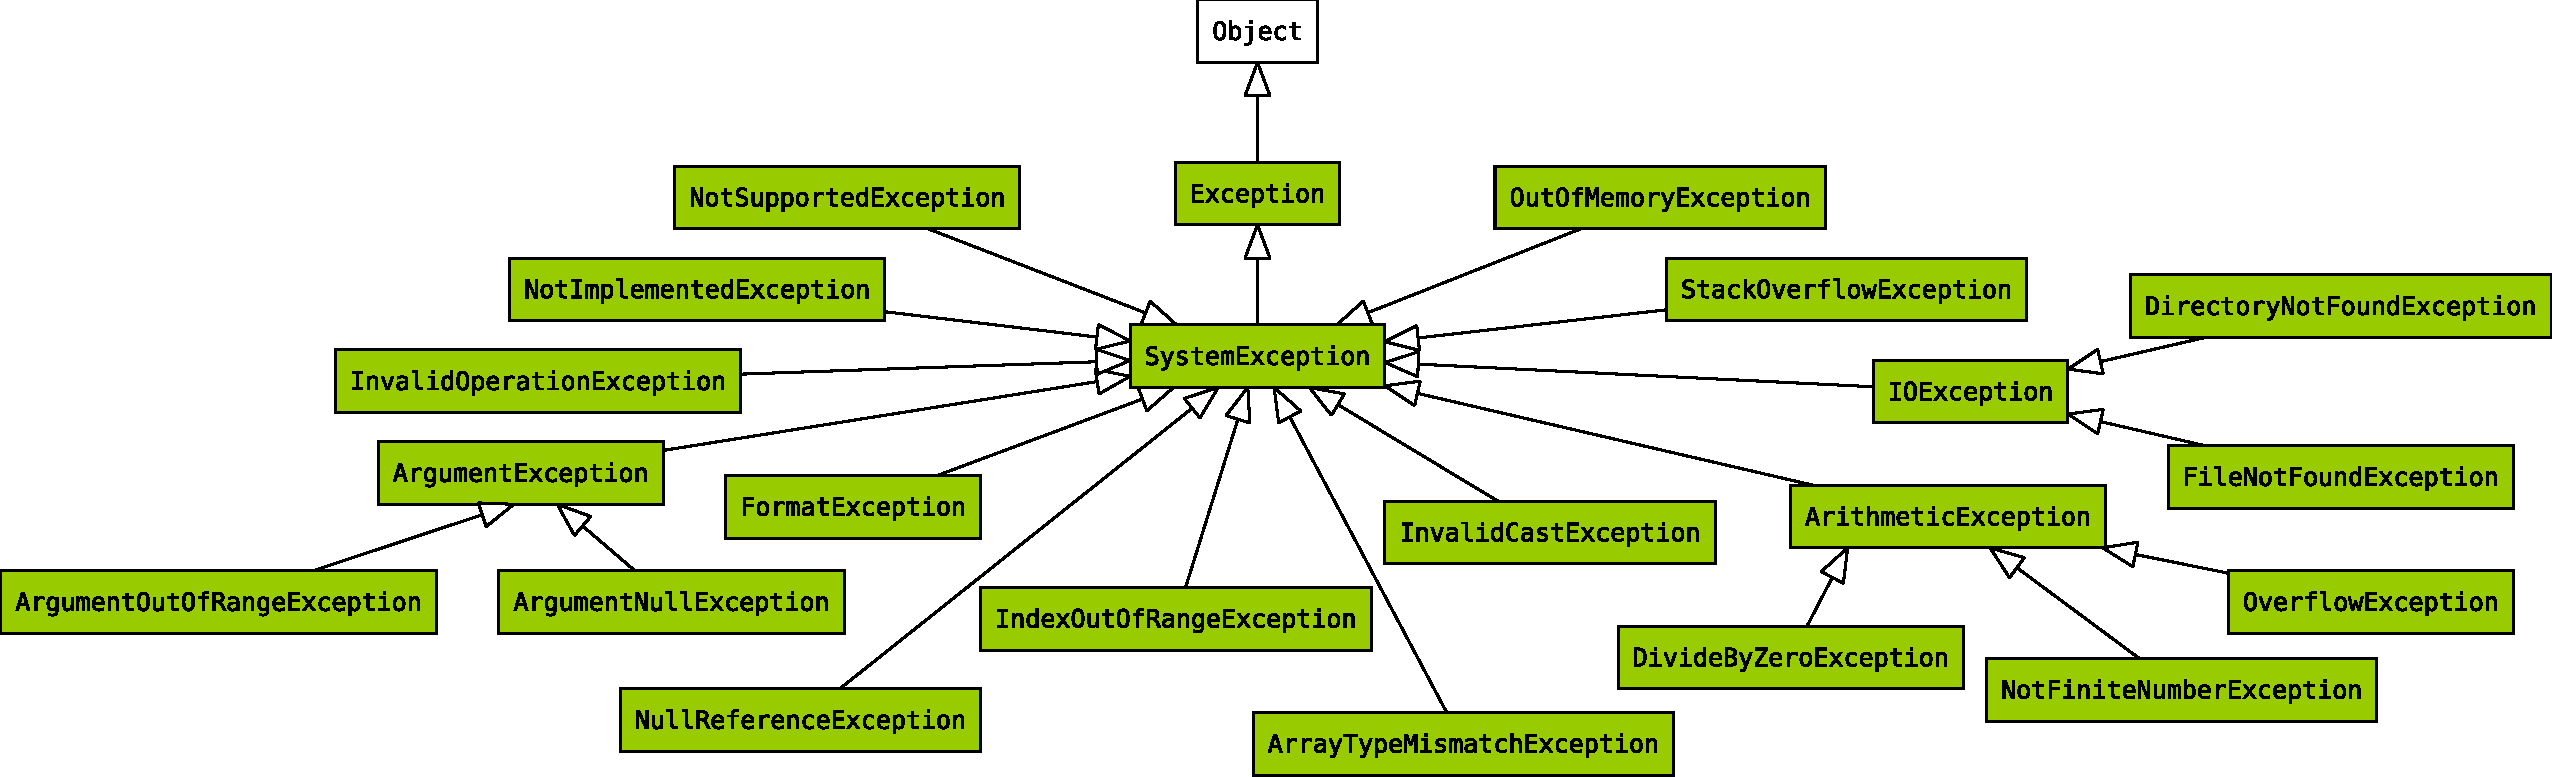
\includegraphics[width=\linewidth]{img/exception-hierarchy.pdf}
\end{frame}


\begin{frame}{The \texttt{throw} Statement}
\begin{block}{What happens on a \cil{throw}?}
  \begin{enumerate}
    \item The control flow is \alert{interrupted}
    \item The control flow is given to any method in the current \alert{call stack} which is capable of \alert{catching} current exception
    \item If none is found, \alert{the program execution is interrupted}
    \item \ldots and the exception's \alert{stack trace} is shown.
  \end{enumerate}
  \end{block}
  \codeview{2}{26}{37}{\tiny}{\codepath{Snippets/ThrowingExceptions.cs}}  
\end{frame}

\begin{frame}{The \texttt{try-catch-finally} Construct}
  \codeview{3}{9}{24}{\tiny}{\codepath{ComplexCatchingException/Program.cs}} 
\end{frame}

\subsection{Generic collections}

\newcommand{\kva}[2]{\alert{\lbrack}\cscat{#1}\alert{\rbrack=}\cscat{#2}}
\newcommand{\kvb}[2]{\alert{\{}\cscat{#1}\alert{,}\cscat{#2}\alert{\}}}


\begin{frame}[allowframebreaks]{Generic Collections and their Type Hierarchy}
  \begin{center}
    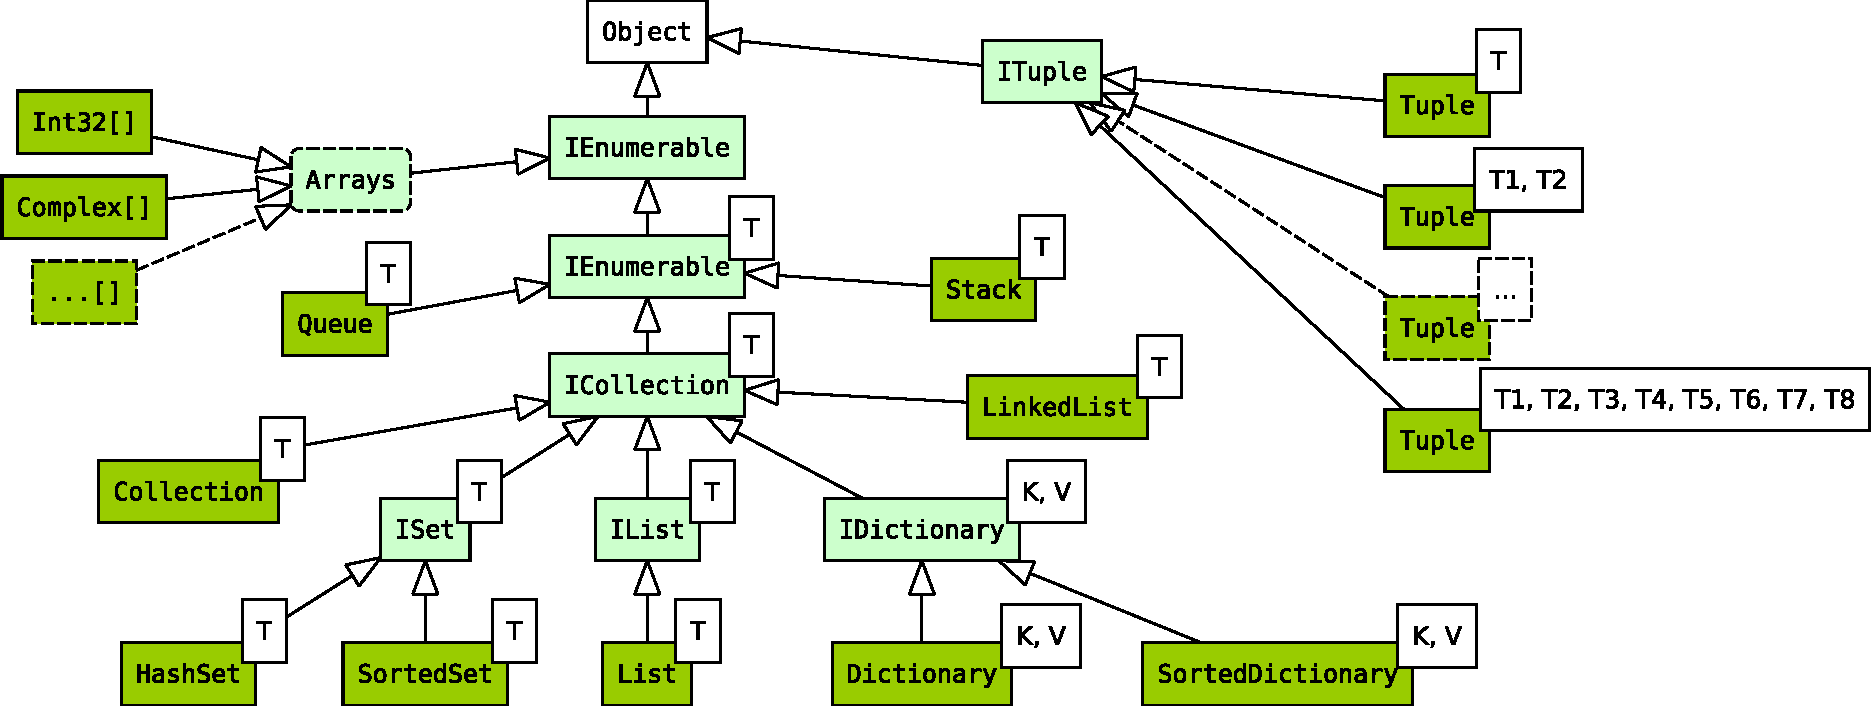
\includegraphics[width=\linewidth]{img/dotnet-collections.pdf}
  \end{center}
  %
  \begin{itemize}
    \item Notice the many \alert{type parameters} (white rectangles)
    \item All dark-green boxes represent classes which can be exploited in everyday programming
  \end{itemize}

  \begin{block}{\texttt{IEnumerable} is the type of all data structures\ldots}
    \begin{center}\itshape
      \ldots containing a number of \alert{\texttt{object}s}, which can be \alert{iterated}
    \end{center}
  \end{block}

  \begin{block}{\texttt{IEnumerable<T>} is the type of all \texttt{IEnumerable}s\ldots}
    \begin{center}\itshape
      \ldots containing a number of instances of \alert{\texttt{T}}, which can be \alert{iterated}
    \end{center}
  \end{block}

  \begin{block}{\texttt{ICollection<T>} is the super-type of all collections}
    Most notably, it is the super-type of:
    %
    \begin{description}
      \item[\texttt{ISet<T>}] i.e. the type of all \alert{sets} whose items are of type \alert{\texttt{T}}
      \item[\texttt{IList<T>}] i.e. the type of all \alert{lists} whose items are of type \alert{\texttt{T}} 
      \item[\texttt{IDictionary<K, V>}] i.e. the type of all \alert{maps} whose \alert{keys} (resp. \alert{values}) are of type \alert{\texttt{K}} (resp. \alert{\texttt{V}})
      %
      \begin{itemize}
        \item in this case \texttt{T} $\equiv$ \texttt{\alert{KeyValuePair<K, V>}}
        \item[ie] a structure defined in \texttt{System.Collections.Generic}
      \end{itemize} 
    \end{description}
  \end{block}

  \begin{block}{\texttt{ITuple} is the super-type of all sorts of tuples}
    Most notably, it is the super-type of:
    %
    \begin{description}
      \item[\texttt{Tuple<T1, T2>}] i.e. the type of all \alert{pairs} whose \alert{first} item is of type \alert{\texttt{T1}} and whose \alert{second} item is of type \alert{\texttt{T2}}
      \item[\texttt{Tuple<T1, T2, T3>}] i.e. the type of all \alert{triples} whose \alert{first} item is of type \alert{\texttt{T1}}, whose \alert{second} item is of type \alert{\texttt{T2}}, whose \alert{third} item is of type \alert{\texttt{T3}}
      \item[\vdots]
    \end{description}
  \end{block}

  \begin{block}{Remarks}
    \begin{itemize}
      \item Most of these types are in \texttt{System.Collections.Generic}
      \item All \alert{sorts} of \alert{arrays} and collections are \alert{enumerable}
      \item Tuples are \alert{not} enumerable
      \item Surprisingly, \texttt{Queue}s, \texttt{Stack}s, and \texttt{LinkedList}s are \alert{not} \texttt{IList}s
      \item Another hierachy exists, rooted in \texttt{ICollection}, for \alert{non-generic} types
      %
      \begin{itemize}
        \item these are contained into \texttt{System.Collections}
      \end{itemize}

      \item Another hierachy exists, rooted in \texttt{IReadOnlyCollection<out T>}, for \alert{read-only} types
      %
      \begin{itemize}
        \item these are contained into \texttt{System.Collections.Generic}
      \end{itemize}

      \item Other types exist, named \texttt{IImmutable*<T>}, for \alert{immutables} types
      %
      \begin{itemize}
        \item these are contained into \texttt{System.Collections.Immutable}
      \end{itemize}
    \end{itemize}
  \end{block}
\end{frame}

\begin{frame}[allowframebreaks]{The \texttt{ICollection<T>} Interface}

  \tcodeview{1}{6}{28}{\tiny}{\codepath{Collections/ICollection.cs}}{The \texttt{System.Collections.Generic.ICollection<T>} Interface}

  \begin{block}{Creation}
    \begin{itemize}
      \item Use the following syntax to provide \alert{items} on the fly:
      %
      \begin{center}\ttfamily
        new \cscat{Collection Class}() \{ \cscat{Item$_1$}, \ldots, \cscat{Item$_N$} \}
      \end{center}
      
      \begin{itemize}
        \item where all \texttt{\cscat{Item$_i$}} are expressions returning instances of \alert{\texttt{T}}
      \end{itemize}
    \end{itemize}
  \end{block}

  \begin{block}{Usage}
    \begin{itemize}
      \item The metods of \texttt{ICollection<T>} support all basic operations
      %
      \begin{itemize}
        \item except directly reading a particular item
      \end{itemize}
      \item By default, they support a \alert{mutable} operation approach
      \item Converting a collection into string \alert{does not shows its items}!
    \end{itemize}
  \end{block}

  \framebreak

  \tcodeview{3}{36}{61}{\tiny}{\codepath{CollectionUsages/Program.cs}}{Creating/Usage example for the \texttt{Collection} class}
  
\end{frame}

\begin{frame}[allowframebreaks]{The \texttt{IList<T>} Interface}

  \tcodeview{1}{6}{23}{\tiny}{\codepath{Collections/IList.cs}}{The \texttt{System.Collections.Generic.IList<T>} Interface}

  
  \framebreak

  \tcodeview{3}{66}{91}{\tiny}{\codepath{CollectionUsages/Program.cs}}{Creating/Usage example for the \texttt{List} class}
  
\end{frame}

\begin{frame}[allowframebreaks]{The \texttt{ISet<T>} Interface}

  \tcodeview{1}{6}{48}{\tiny}{\codepath{Collections/ISet.cs}}{The \texttt{System.Collections.Generic.ISet<T>} Interface}

  \framebreak

  \tcodeview{3}{96}{119}{\tiny}{\codepath{CollectionUsages/Program.cs}}{Creating/Usage example for the \texttt{HashSet} class}
  %
  \begin{itemize}
    \item consider retrying the same test with the \texttt{SortedSet<T>} class
  \end{itemize}

\end{frame}

\begin{frame}[allowframebreaks]{The \texttt{IDictionary<K, V>} Interface}

  \tcodeview{1}{6}{29}{\tiny}{\codepath{Collections/IDictionary.cs}}{The \texttt{System.Collections.Generic.IDictionary<K, V>} Interface}

  
  \framebreak

  \tcodeview{3}{124}{163}{\tiny}{\codepath{CollectionUsages/Program.cs}}{Creating/Usage example for the \texttt{Dictionary} class}
  %
  \begin{itemize}
    \item consider retrying the same test with the \texttt{SortedDictionary<K, V>} class
  \end{itemize}

\end{frame}

\begin{frame}[allowframebreaks]{The \texttt{Tuple<T1, T2, ...>} Classes}

  \tcodeview{1}{3}{23}{\tiny}{\codepath{Collections/Tuple.cs}}{The \texttt{System.Tuple<T1, T2, ...>} Class}

  
  \framebreak

  \tcodeview{3}{168}{185}{\tiny}{\codepath{CollectionUsages/Program.cs}}{Creating/Usage example for the \texttt{Dictionary} class}

\end{frame}

\section{Functional programming in C\#}
\renewcommand{\codepath}[1]{../../code/lecture-07/#1}

\fr{Improving functional strategies}{
    \bl{Functional strategies}{\iz{
        \item a specific case of the so-called Strategy pattern
        \item methods/constructors accept arguments of an interface with just one method, one or more implementing classes, the need of creating an object when the strategy is to be defined
        \item the whole idea is actually simply that of a ``function''
    }}
    \bl{The C\# path across time: how to instantiate a delegate}{\iz{
        \item wrapping method references (C\# 1.0)
        \item anonymous functions (C\# 2.0)
        \item lambdas (C\# 3.0) -- the one suggested now
    }}
}

\frs{10}{Consider a \Cil{BankAccount}}{
  \bl{With methods for:}{\iz{
    \item withdrawing
    \item checking balance
  }}
  \bl{Abstracting a \cil{IFeeCalculator}}{\iz{
    \item the hypothesis that withdrawal fee is $1$ appears weak
    \item surely this has to be generalise
    \item it could vary across different accounts
    \item it could vary dependning on the actual amount
    \item could introduce an interface \cil{IFeeCalculator}
  }}
  \bl{Abstracting a \cil{IWithdrawalAction}}{\iz{
    \item what should we do if withdrawal fail?
    \item surely that task is better left to a different class
    \item in this case, perhaps many different behaviour have to be defined
    \item shuold abstract from that specific behaviour
    \item could introduce an interface \cil{IWithdrawalAction}
  }}
  
}


\fr{Interfaces}{
  \codeview{1}{14}{44}{\tiny}{\codepath{BankAccountStrategies/Program.cs}}
}

\fr{\Cil{FlexibleBankAccount}}{
  \codeview{1}{46}{75}{\tiny}{\codepath{BankAccountStrategies/Program.cs}}
}

\fr{\Cil{UseFlexibleBankAccount}}{
  \codeview{1}{77}{98}{\tiny}{\codepath{BankAccountStrategies/Program.cs}}
}


\frs{10}{C\# delegates}{
    \bl{Delegate}{\iz{
        \item a delegate is a wrapper for a method (reference) of a specific type (input/output arguments)
        \item defining a delegate \cil{D} means to define one such type and giving it a name
        \item syntax: \cil{delegate <ret-type> D(<parameters list>);}
        \item ``under the hood'' this is just a subclass of \cil{System.Delegate}
    }}
    \bl{Instantiation of a delegate by method reference}{\iz{
        \item if there is a method \cil{M} (static or instance) accessible in scope
        \item you can define a variable of type \cil{D} assigned to method \cil{M}
        \item syntax: \cil{D del = new D(M);}, or simply passing \cil{M} where a \cil{D} is expected
    }}
    \bl{Call of a delegate}{\iz{
        \item given the above definition, simply \cil{del} is like a method to be called
    }}
    \bl{Multichannel delegates}{\iz{
        \item given two delegates that return void (also called \alert{even delegates}), they can be combined by operators \cil{+}, \cil{-}, \cil{+=}, \cil{-=}
    }}
}


\fr{Definition and use of delegates}{
  \codeview{1}{13}{43}{\tiny}{\codepath{BankAccountDelegates/Program.cs}}
}

\fr{Instantiation of delegates}{
  \codeview{1}{45}{75}{\tiny}{\codepath{BankAccountDelegates/Program.cs}}
}

\fr{Anonymous functions}{
    \bl{Pros and cons of delegates}{\iz{
        \item surely reduce boilerplace code, and are hence more convenient than using interfaces
        \item still there's boilerplate code, since a method is needed somewhere to implement your functional strategy, even if short
        \item recalling that a functional strategy is just a ``function'' (in a mathematical/computational interpretation)...
        
    }}
    \bl{Anonynous functions}{\iz{
        \item a mechanism to express ``in-line'' a function to be passed where a delegate is expected
        \item syntax of expression: \cil{delegate(<parameters list>)\{<body>\}}, to be passed where a compatible delegate is expected
        \item essentially, it is a function without name and with keyword \cil{delegate} upfront
    }}
}

\fr{Using anonymous function}{
  \codeview{1}{16}{47}{\tiny}{\codepath{BankAccountAnonymous/Program.cs}}
}

\frs{5}{Lambda expressions}{
    \bl{Pros and cons of anonymous functions}{\iz{
        \item surely further reduce boilerplace code, and are hence more convenient than using method references
        \item still there's boilerplate code, since the syntax is still rather long: one would more heavility rely on inference and on single-expression body
        \item lambda-expressions have been invented in 1930 by Alonso Church
        \item Scala language started using them in OOP languages, and now also Java have them
    }}
    \bl{Lambda-expression}{\iz{
        \item Complete syntax: \cil{(T1 x1,...,Tn xn) => \{<body>\}}
        \item With inference: \cil{(x1,...,xn) => \{<body>\}}
        \item With single-expression body: \cil{(T1 x1,...,Tn xn) => <exp>}
        \item With single argument and inference: \cil{x => \{<body>\}}
        \item With unused inputs: \cil{(_,...,_) => \{<body>\}}
        \item ...and combinations
        \item[$\Rightarrow$] should generally use the shortest version possible
    }}
}

\fr{Using lambdas}{
  \codeview{1}{9}{37}{\tiny}{\codepath{BankAccountLambdas/Program.cs}}
}

\frs{10}{Reusable delegates in libraries}{
    \bl{Generic functions in namespace \cil{System}}{\iz{
        \item \cil{delegate TResult Func<out TResult>(); }
        \item \cil{delegate TResult Func<in T, out TResult(T arg); }
        \item \cil{delegate TResult Func<in T1, in T2, out TResult(T1 arg1, T2 arg2); }
        \item \dots
        \item \cil{delegate bool Predicare<in T>(T obj)}
    }}
    \bl{Generic actions in namespace \cil{System}}{\iz{
        \item \cil{delegate void Action(); }
        \item \cil{delegate void Action<in T>(T obj); }
        \item \cil{delegate void Action<in T1, in T2>(T1 obj1, T2 obj2); }
        \item \dots
    }}
    \bl{Guideline}{\iz{
        \item define your own delegates only if domain-specific
        \item otherwise, consider using  library delegates
    }}
}

\fr{\Cil{BankAccount} with \Cil{Func} and \Cil{Action}}{
  \codeview{1}{14}{40}{\tiny}{\codepath{BankAccountFunc/Program.cs}}
}

\fr{Use \Cil{BankAccount} with \Cil{Func} and \Cil{Action}}{
  \codeview{1}{42}{66}{\tiny}{\codepath{BankAccountFunc/Program.cs}}
}

\fr{Exercise with \Cil{Func}, \Cil{Predicate} and \Cil{Action}}{
  \codeview{1}{7}{35}{\tiny}{\codepath{ExercisesWithFunc/Program.cs}}
}

\fr{Solution for the first three}{
  \codeview{1}{37}{59}{\tiny}{\codepath{ExercisesWithFunc/Program.cs}}
}

\fr{Expectations}{
  \codeview{1}{61}{81}{\tiny}{\codepath{ExercisesWithFunc/Program.cs}}
}


\fr{A preview of standard LINQ library}{
    \codeview{1}{28}{56}{\tiny}{\codepath{LINQExample/Program.cs}}
}

\fr{The used \Cil{Person} class}{
  \codeview{1}{7}{26}{\tiny}{\codepath{LINQExample/Program.cs}}
}


\end{document}
